\section{Laboratory work implementation}

\subsection{Tasks and Points}
I chosed The Advanced Level for my Labrotory work.
\begin{itemize}
\item Create a Windows application
\item Add 2 buttons to window: one with default styles, one with custom style.
\item Add 2 text elements to window: one with default style , one with custom style.
\item Make elements to interact or change other elements
\item Change behavior of different window actions (for example onclick close window move window to a random location)
\end{itemize}
\subsection{Laboratory work analysis}

https://github.com/szraksy/WP

Firstable i created a window on Visual Studio and put 2 text labels ,2
textboxes, 2 buttons. One of them 2 labels is Custom with blue color. The
other one has standard still.
One of them 2 textboxes is standard still and the other one has a
background color with gray and the text color is White.
One of them 2 buttons is standard still and the other one is custom still
with red background color and White text color.
To the first step the custom button can be clickable but standard button
can not be clickable. When you click the custom button then the situation
will be oppisite.
I added some action with button on my program. For example when we
click the custom button which is the red background ,then we will see
background of the textboxes color change. And there will be appeare a
popup window which is saying “You changed to the custom still” and the
custom button will be non clickable.
And when we click the standard button then the popup will appeare again
and it shows us a message “You changed to standard still” and custom
button will be clickable the standard button will be non clickable.
Also, i changed the background color with custom button.


\subsection{Prove your work with screens}

\begin{figure}
	\centering
	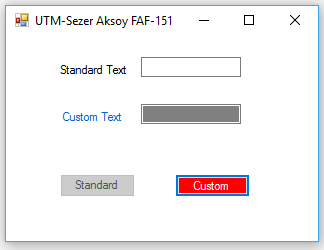
\includegraphics[width=0.7\linewidth]{first.PNG}
	\caption{}
	\label{fig:first}
\end{figure}

\begin{figure}
	\centering
	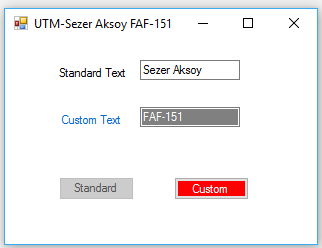
\includegraphics[width=0.7\linewidth]{second.PNG}
	\caption{}
	\label{fig:second}
\end{figure}

\begin{figure}
	\centering
	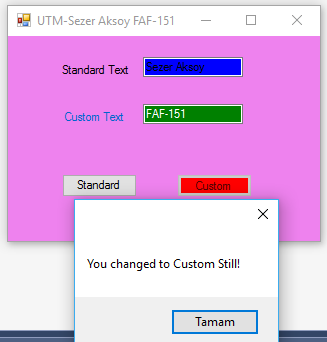
\includegraphics[width=0.7\linewidth]{thirth.PNG}
	\caption{}
	\label{fig:thirth}
\end{figure}

\begin{figure}
	\centering
	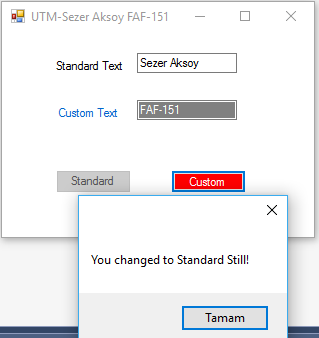
\includegraphics[width=0.7\linewidth]{fourth.PNG}
	\caption{}
	\label{fig:fourth}
\end{figure}


\clearpage